%@AUTHOR: Cardel
%Configuracion del documento

\documentclass{beamer}
\usetheme{Berkeley}
\setbeamertemplate{caption}[numbered]
\usepackage{graphicx}
\usepackage[utf8]{inputenc}
\usepackage[spanish]{babel}
\usepackage{ragged2e}
\usepackage{colortbl}
\usepackage{color}
\definecolor{naranja}{rgb}{1,0.5,0} % valores de las componentes roja, verde y azul (RGB)
\definecolor{rojo}{rgb}{1,0,0}
\definecolor{SteelBlue}{rgb}{0.3,0.5,0.7}
\usepackage{float}

\author{Carlos Andr\'es Delgado S.} 
\title{710193M Arquitectura de computadores II}
\subtitle{Unidad de control \\ carlos.andres.delgado@correounivalle.edu.co}
\institute{Facultad de Ingeniería. Universidad del Valle}
%Transparencia
\setbeamercovered{transparent}

%LOGO Univalle
\pgfdeclareimage[height=1.4cm]{logo}{imagenes/univalle}
\logo{\pgfuseimage{logo}}

\usepackage{listings}% http://ctan.org/pkg/listings
\usepackage{listingsutf8}

\lstset{ %
  basicstyle=\footnotesize,           % the size of the fonts that are used for the code
  numbers=none,
  numberstyle=\footnotesize,          % the size of the fonts that are used for the line-numbers
  numbersep=4pt,                  % how far the line-numbers are from the code
  backgroundcolor=\color{white},      % choose the background color. You must add \usepackage{color}
  breaklines=true,                % sets automatic line breaking
  breakatwhitespace=true,        % sets if automatic breaks should only happen at whitespace
  title=\lstname,                   % show the filename of files included with \lstinputlisting;{}
  extendedchars=false,
  inputencoding=utf8, 
  tabsize=2,
   mathescape=true,
  literate={\ \ }{{\ }}1
}
\newsavebox{\myLst}
\newsavebox{\myLstb}
\newsavebox{\myLstc}
\newsavebox{\myLstd}

\usepackage{enumitem} % enumerados

%Para que en cada seccion aparezca la tabla de contenido
\AtBeginSection[]{
	\begin{frame}
	\frametitle{Contenido}
	\tableofcontents[currentsection]
\end{frame}
}




\date{Mayo de 2016}
\newcommand{\grad}{\hspace{-2mm}$\phantom{a}^{\circ}$}
\begin{document}

\begin{frame}
	\titlepage	 		
\end{frame}

\begin{frame}
	\tableofcontents	 		
\end{frame}


\section{Microoperaciones}

\begin{frame}
	\frametitle{Microoperaciones}
	\begin{block}{Conceptos}
	Cuando se ejecuta un programa se tienen una secuencia de ciclos de captación y ejecución para cada instrucción. Sin embargo, estas operaciones pueden descomponerse en operaciones más pequeñas.
	\end{block}		 		
	\begin{figure}[H]
		\centering
		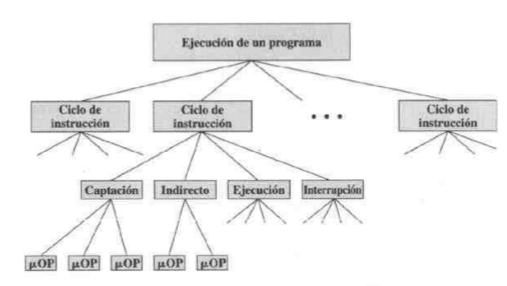
\includegraphics[scale=0.4]{imagenes/programa.png} 
	\end{figure}
\end{frame}

\begin{frame}
	\frametitle{Microoperaciones}
	\begin{block}{Ciclo de captación}
	Se examina el ciclo de captación, que tiene lugar al principio de cada instrucción, el cual involucra los siguientes registros del procesador
	\begin{enumerate}
		\item \textbf{Registro de dirección de memoria (MAR)} Está conectado a las líneas de dirección del bus
		\item \textbf{Registro intermedio de memoria (MBR)} Está conectado a las líneas de datos del bus
		\item \textbf{Contador de programa (PC)} Contiene la dirección a la siguiente instrucción a captar
		\item \textbf{Registro de instrucción (IR)} Contiene la última instrucción captada
	\end{enumerate}	 
	\end{block}
\end{frame}

\begin{frame}
	\frametitle{Microoperaciones}
	\begin{block}{Ciclo de captación}
	El proceso puede ser estudiado en las siguientes unidades de tiempo
	\begin{enumerate}
		\item \textbf{Primera unidad de tiempo:} Transferir PC a MAR
		\item \textbf{Segunda unidad de tiempo:} Direccionar en la memoria (MAR) y almacenar en MBR e incrementar PC
		\item \textbf{Tercer unidad de tiempo:} Transferir de MBR a IR (Instrucción a ejecutar)
	\end{enumerate}	 
	\end{block}
\end{frame}


\begin{frame}
	\frametitle{Microoperaciones}
	\begin{block}{Ciclo indirecto}
	Una vez se capta una instrucción, el siguiente paso es captar los operandos fuente. Las microperaciones requeridas son.
	\begin{enumerate}
		\item \textbf{Primera unidad de tiempo:} Transferir a MAR la dirección del operando
		\item \textbf{Segunda unidad de tiempo:} Direccionar en la memoria (MAR) y almacenar en MBR e incrementar PC
		\item \textbf{Tercer unidad de tiempo:} Transferir de MBR a IR (Instrucción a ejecutar)
	\end{enumerate}	 
	\end{block}
\end{frame}

\begin{frame}
	\frametitle{Microoperaciones}
	\begin{block}{Ciclo de interrupción}
	Este se presenta cuando hemos tenido una señal de interrupción durante la ejecución de la instrucción.
	\begin{enumerate}
		\item \textbf{Primera unidad de tiempo:} Transferir a MBR el valor de PC
		\item \textbf{Segunda unidad de tiempo:} Transferir a MAR la dirección donde quedamos al momento de llegar la interrupción. PC ahora tiene la dirección de la instrucción de la interrupción
		\item \textbf{Tercer unidad de tiempo:} Tranferir a memoria el valor de MBR (Guardar el contexto)	
	\end{enumerate}	 
	\end{block}
\end{frame}

\begin{frame}
	\frametitle{Microoperaciones}
	\begin{block}{Ciclo de ejecución}
	Es más complejo ya que depende de las operaciones se requieran hacer en el procesador. Las microoperaciones dependen de:
	\begin{enumerate}
		\item Número de operadores se requieren en la instrucción
		\item Si se requiere almacenamiento temporal durante la ejecución
		\item Donde se almacena el resultado de la operación	
	\end{enumerate}	 
	\end{block}
\end{frame}



\section{Control del procesador}

\begin{frame}
	\frametitle{Control del procesador}
	\begin{block}{Requisitos funcionales}
	De acuerdo a lo visto anteriormente, se han descompuesto las instrucciones en microperaciones o operaciones elementales. Por ello se deben definir los requisitos funcionales de la unidad de control del procesador y por ello, se debe realizar la caracterización del procesador:
	\begin{enumerate}
		\item Definir elementos básicos del procesador
		\item Describir las microoperaciones del procesador
		\item ¿Que debe hacer la unidad de control para que el procesador haga las microoperaciones?
	\end{enumerate}	 
	\end{block}
\end{frame}

\begin{frame}
	\frametitle{Control del procesador}
	\begin{block}{Requisitos funcionales}
	Las microperaciones de un procesador se pueden clasificar de la siguiente forma:
	\begin{enumerate}
		\item Transferir datos en un registro a otro
		\item Transferir datos de un registro a un E/S
		\item Transferir datos de E/S a un registro
		\item Realizar alguna operación (arimética o lógica)
	\end{enumerate}	 
	\end{block}
\end{frame}

\begin{frame}
	\frametitle{Control del procesador}
	\begin{block}{Requisitos funcionales}
	La unidad de control realiza dos tareas básicas:
	\begin{enumerate}
		\item \textbf{Secuenciamiento:} Hace que el procesador avance a través de una serie de microoperaciones para realizar alguna tarea
		\item \textbf{Ejecución:} Hace que ejecute cada micropoperación
	\end{enumerate}	 
	\end{block}
\end{frame}

\begin{frame}
	\frametitle{Control del procesador}
	\begin{block}{Señales de control}
	Son aquellas señales para controlar los elementos en el procesador
	\begin{enumerate}
		\item \textbf{Reloj:} Para sincronizar los elementos del procesador
		\item \textbf{Registro de instrucción:} Código de la operación a realizar
		\item \textbf{Indicadores:} Banderas de estado del procesador
		\item \textbf{Señales del bus de control:} Manejar las señales de interrupción
		\item \textbf{Señales de control internas del procesador:} Registros y ALU
		\item \textbf{Señales de control hacia el bus de control:} Memoria y E/S
	\end{enumerate}	 
	\end{block}
\end{frame}

\begin{frame}
	\frametitle{Control del procesador}
	\begin{block}{Señales de control}
	Esquema de señales de control:
	\end{block}		 		
	\begin{figure}[H]
		\centering
		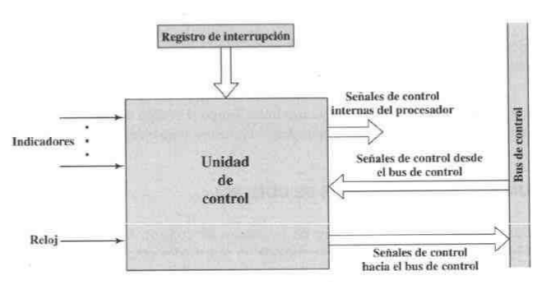
\includegraphics[scale=0.4]{imagenes/control.png} 
	\end{figure}
\end{frame}


\section{Implementación cableada}


\begin{frame}
	\frametitle{Implementación cableada}
	\begin{block}{Organización interna del procesador}
	Para que la unidad de control sea funcional, deben conectarse todas las señales hacia los elementos de la CPU y el bus de control. Existen dos tipos de implementación:
	\begin{enumerate}
		\item Implementación cableada
		\item Implementación microprogramada
	\end{enumerate}
	\end{block}
\end{frame}


\begin{frame}
	\frametitle{Implementación cableada}
	\begin{block}{Entradas de la unidad de control}
	Las entradas de la unidad de control son el reloj, los indicadores, el registro de instrucción y las líneas de control del bus. Estas pueden ser vistas como una secuencia de bits y estas pueden ser codificadas como una línea de $n$ bits. Por ello, es util utilizar un decodificador de $n$ entradas y $2^n$ salidas. Con ello se garantiza:
	\begin{enumerate}
		\item Sólo se activa una línea en la salida ante un estimulo de entrada
		\item Se pueden identificar las instrucciones claramente
	\end{enumerate}
	\end{block}
\end{frame}

\begin{frame}
	\frametitle{Implementación cableada}
	\begin{block}{Entradas de la unidad de control}
	Esquema de cableado de señales de control:
	\end{block}		 		
	\begin{figure}[H]
		\centering
		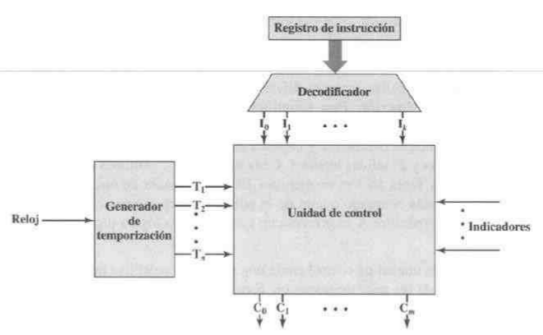
\includegraphics[scale=0.4]{imagenes/controlsignal.png} 
	\end{figure}
\end{frame}

 
\begin{frame}
	\frametitle{Preguntas}
	\vfill
	\begin{center}
	¿Preguntas?\\
	\vfill
	Siguiente tema: \\
	Control microprogramado
	\end{center}
\end{frame}


\end{document}